\documentclass[10pt, landscape]{article}
\usepackage[scaled=0.92]{helvet}
\usepackage{calc}
\usepackage{multicol}
\usepackage{ifthen}
\usepackage[a4paper,margin=3mm,landscape]{geometry}
\usepackage{amsmath,amsthm,amsfonts,amssymb}
\usepackage{color,graphicx,overpic}
\usepackage{hyperref}
\usepackage{newtxtext} 
\usepackage{enumitem}
\usepackage{amssymb}
\usepackage[table]{xcolor}
\usepackage{vwcol}
\usepackage{tikz}
\usetikzlibrary{arrows.meta}
\usetikzlibrary{calc}
\usepackage{mathtools}
\usepackage{nicematrix}
%For pictures / figures
\usepackage{color,graphicx,overpic}
\graphicspath{ {./images/} }
% for relations
\usepackage{cancel}
\usepackage{ mathrsfs }
\graphicspath{ {./images/} }
\setlist{nosep}

\pdfinfo{
  /Title (MA1512.pdf)
  /Creator (TeX)
  /Producer (pdfTeX 1.40.0)
  /Author (Seamus)
  /Subject (Example)
  /Keywords (pdflatex, latex,pdftex,tex)}

% Turn off header and footer
\pagestyle{empty}

\newenvironment{tightcenter}{%
  \setlength\topsep{0pt}
  \setlength\parskip{0pt}
  \begin{center}
}{%
  \end{center}
}

% redefine section commands to use less space
\makeatletter
\renewcommand{\section}{\@startsection{section}{1}{0mm}%
                                {-1ex plus -.5ex minus -.2ex}%
                                {0.5ex plus .2ex}%x
                                {\normalfont\large\bfseries}}
\renewcommand{\subsection}{\@startsection{subsection}{2}{0mm}%
                                {-1explus -.5ex minus -.2ex}%
                                {0.5ex plus .2ex}%
                                {\normalfont\normalsize\bfseries}}
\renewcommand{\subsubsection}{\@startsection{subsubsection}{3}{0mm}%
                                {-1ex plus -.5ex minus -.2ex}%
                                {1ex plus .2ex}%
                                {\normalfont\small\bfseries}}%
\renewcommand{\familydefault}{\sfdefault}
\renewcommand\rmdefault{\sfdefault}
% makes nested numbering (e.g. 1.1.1, 1.1.2, etc)
\renewcommand{\labelenumii}{\theenumii}
\renewcommand{\theenumii}{\theenumi.\arabic{enumii}.}
\renewcommand\labelitemii{•}
%  for logical not operator
\renewcommand{\lnot}{\mathord{\sim}}
\renewcommand{\bf}[1]{\textbf{#1}}
\newcommand{\abs}[1]{\vert #1 \vert}
\newcommand{\Mod}[1]{\ \mathrm{mod}\ #1}

\makeatother
\definecolor{myblue}{cmyk}{1,.72,0,.38}
\everymath\expandafter{\the\everymath \color{myblue}}
% Define BibTeX command
\def\BibTeX{{\rm B\kern-.05em{\sc i\kern-.025em b}\kern-.08em
    T\kern-.1667em\lower.7ex\hbox{E}\kern-.125emX}}
\let\iff\leftrightarrow
\let\Iff\Leftrightarrow
\let\then\rightarrow
\let\Then\Rightarrow

% Don't print section numbers
\setcounter{secnumdepth}{0}

\setlength{\parindent}{0pt}
\setlength{\parskip}{0pt plus 0.5ex}
%% this changes all items (enumerate and itemize)
\setlength{\leftmargini}{0.5cm}
\setlength{\leftmarginii}{0.5cm}
\setlist[itemize,1]{leftmargin=2mm,labelindent=1mm,labelsep=1mm}
\setlist[itemize,2]{leftmargin=4mm,labelindent=1mm,labelsep=1mm}

%My Environments
\newtheorem{example}[section]{Example}
% -----------------------------------------------------------------------

\begin{document}
\raggedright
\footnotesize
\begin{multicols}{4}


% multicol parameters
% These lengths are set only within the two main columns
\setlength{\columnseprule}{0.25pt}
\setlength{\premulticols}{1pt}
\setlength{\postmulticols}{1pt}
\setlength{\multicolsep}{1pt}
\setlength{\columnsep}{2pt}

\begin{center}
    \fbox{%
        \parbox{0.8\linewidth}{\centering \textcolor{black}{
            {\Large\textbf{MA1512}}
            \\ \normalsize{AY24/25 sem 1}}
            \\ {\footnotesize \textcolor{myblue}{github.com/mendax1234}} 
        }%
    }
\end{center}

\section{01. Introduction to Differential Equations}
\subsection{First Principles}
\begin{enumerate}
    \item (\textbf{Differential Equation}) Let $x$ be an independent variable and $y$ be a dependent variable. An equation that involves $x,y$ and \textbf{various derivatives of $y$} is called a \textbf{differential equation}. e.g. $(\frac{dy}{dx})^3+e^x+2=\frac{d^2y}{dx^2}$
    \item (\textbf{Ordinary Differential Equation}) In general, an equation of the form $F(x,y,\frac{dy}{dx}, \cdots, \frac{d^ny}{dx^n})=0$ is an \textbf{ordinary differential equation}. It is called so because there is only \textbf{one} independent variable and only \textbf{ordinary derivatives (not partial derivatives)} are involved.
    \item (\textbf{Order of a Differential Equation}) The \textbf{order} of a differential equation is the order of the \textbf{highest derivative} appearing in the differential equation. e.g. $dy/dx$ is first order derivative, $d^2y/dx^2$ is second order derivative.
    \item (\textbf{Solution of a Differential Equation})
    \begin{itemize} 
        \item (\textbf{General Solution}) A \textbf{general solution} to a differential equation is a family of infinitely many possible solutions, often involving \textbf{arbitrary constants} and they satisfy the differential equation when they are substituted into the differential equation.
        \item (\textbf{Particular Solution}) With additional information such as \textit{initial condition} (where a differential equation is required to satisfy conditions on the dependent variable and its derivatives specified at one value of the independent variable), we can determine a \textbf{particular solution} that no longer involves arbitrary constants.
    \end{itemize}
    Note that the solution can be in \textbf{implicit form}.
    \item (\textbf{The method of separation of variables}) A first-order differential equation of the form $\frac{dy}{dx}=F(x,y)$ is \textbf{separable} if it can be written as $M(x)dx=N(y)dy$. To solve this, directly integrate both sides of the equation, we will get $\int N(y)dy=\int M(x)dx+C$, where $C$ is an arbitrary constant.
    \begin{itemize}
        \item (\textbf{The position of arbitrary constant $C$}) The arbitrary constant must be added immediately when you integrate w.r.t independent variable.
        \item (\textbf{Notation}) Sometimes $dy/dx$ is written simply as $y'$.
        \item (\textbf{Some useful substitution})
        \begin{itemize}
            \item If $y'=f(ax+by+c)$, we employ a \textit{linear change of variable}. Let $u=ax+by+c\rightarrow u'=a+by'$
            \item If $y'=f(y/x)$, we let $y=xv$, and $y'=xv'+v$ (Chain Rule) (This is same as let $v=\frac{y}{x}$ first.
        \end{itemize}
        Note that in both substitutions, we assume the function at the right side can be written as $f(\cdots)$, which is the soul in substitution.
    \end{itemize}
    \item (\textbf{Classic Examples})
    \begin{itemize}
        \item (\textbf{Half-Life}) The typical scenario for half-life is \textit{exponential decay}, in which we have $\frac{dx}{dt}=-kx,k>0$ and since its solution is $x=x_0e^{-kt}$. We can get the formula to determine the \textit{decay rate $k$} given that we know the half-life $\tau$, so, it will be $\frac{x_0}{2}=x_0e^{-kt}\rightarrow k=\frac{ln2}{\tau}$
        \item Remember that $\int\frac{2u+4}{u^2+4u+5}=\ln(u^2+4u+5)$.
        \item For $y'\cdot y''=2$, to use separation of variables, use substitution $u=y'\rightarrow u\cdot u'=2$ Then solve it accordingly.
    \end{itemize}
\end{enumerate}
\subsection{The Geometry of Differential Equations}
\begin{enumerate}
    \item (\textbf{Geometry of First-Order Differential Equation}) Note that $y'$ is the slope of curve $y=y(x)$ on the $x-y$ plane. Hence, solving differential equation $y'=f(x,y)$ means \textbf{finding curves whose slope at any given point $(x,y)$ is equal to $f(x,y)$}. If adding initial value condition $y(x_0)=y_0$, that means the curve must pass through $(x_0, y_0)$.
    \item (\textbf{Using Direction/Slope Field to understand}) $\cdots$ \textbf{finding curves that are tangent to the short straight line at each point $(x,y)$}. If adding initial value condition $y(x_0)=y_0$, that means the curve must pass through $(x_0, y_0)$.
    \item (\textbf{Equilibrium Solution}) An \textbf{equilibrium solution} of a differential equation is a solution that is \textbf{constant} ($y(t)=\beta$); these correspond to \textbf{horizontal lines} on a direction field (can have multiple equilibrium solutions).
    \begin{itemize}
        \item (\textbf{Stable Equilibrium Solution}) An equilibrium solution $y(t)=\beta$ is said to be \textbf{stable} if solutions about/near this equilibrium approach $\beta$ as $t\to \infty$.
        \item (\textbf{Unstable Equilibrium Solution)} Otherwise, the equilibrium point is said to be \textbf{unstable}.
    \end{itemize}
    \item (\textbf{Methods to find equilibrium solution})
    \begin{itemize}
        \item Judge the order of the diff eq and let all the dependent variables' derivatives to be 0. e.g. First order $\rightarrow y'=0$, Second order $\rightarrow y'=0 \text{ and } y''=0$. e.g. $y'=-10y(20-y)(1-\frac{1}{30}y)\rightarrow 0=-10y(20-y)(1-\frac{1}{30}y)$
        \item Use basic inequality technique to solve and sketch out a sign diagram for $dy/dt$ with $y$ For example,\\
        \centerline{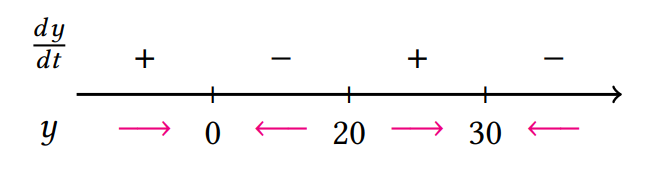
\includegraphics[width=0.9\linewidth]{image/sign-diagram-for-dydt.png}}
        \item Draw the corresponding direction/slope field to judge the stability. For example,\\
        \centerline{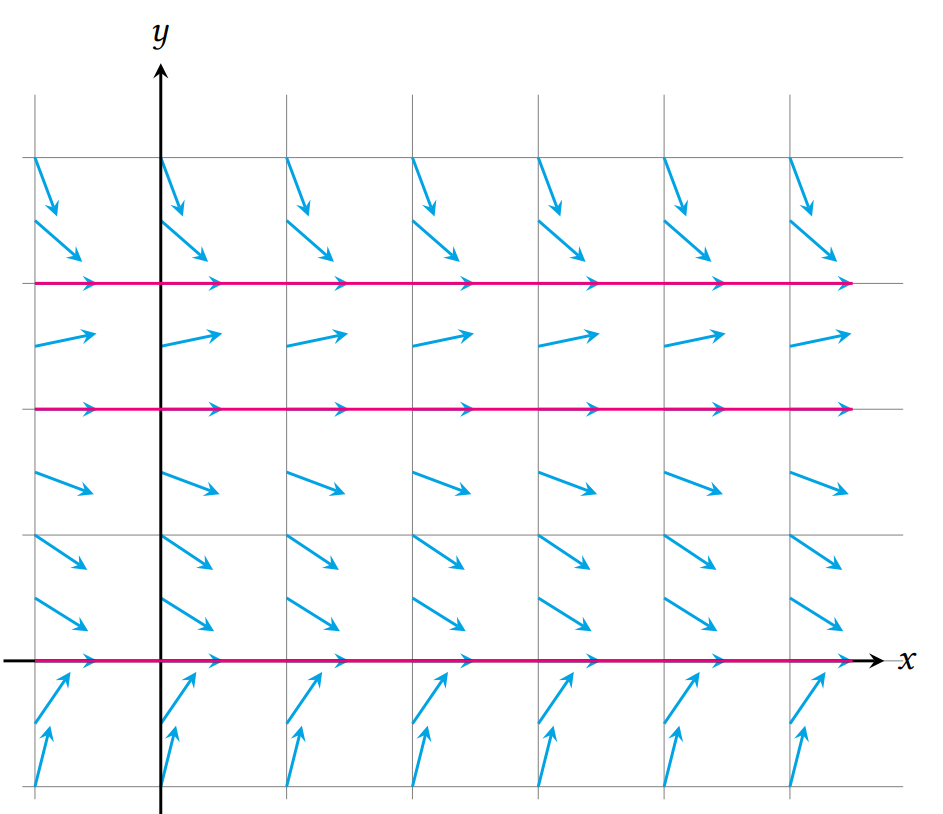
\includegraphics[width=0.5\linewidth]{image/direction-field.png}}
    \end{itemize}
\end{enumerate}
\subsection{Population Dynamics}
\begin{enumerate}
    \item (\textbf{Malthusian model}) It assumes that the rate of change of a population is proportional to its present value. That is $dy/dt=ky\rightarrow y(t)=y_0e^{kt}$, where $y_0=y(0)$. This model suggests that a population would grow exponentially with \textbf{growth rate} k. (\textbf{Note that in Malthusan model, it is $y=y_0\cdot e^{kt}$, however, in half-life model, it is $x=x_0\cdot e^{-kt}$})
    \item (\textbf{Verhulst model}) In Verhulst, our \textbf{growth rate} varies according to the present value $y$ of the population. The formula is given by $\frac{dy}{dt}=[k(1-\frac{y}{y_\infty})]y$, where $dy/dt$ is \textbf{rate of change} and $k(1-y/y_\infty)$ is \textbf{growth rate}. This model assumes that a population grows \textbf{logistically}, such that given any initial population, $lim_{t\to \infty}y(t)=y_\infty$, and $y_\infty$ is called the \textit{carrying capacity}.
    \item (\textbf{Hunt rate}) Since hunt rate(E) is usually given in constant number per period, and in both models we have rate of change $dy/dt$, so usually we just minus the hunt rate (E) at the right side of our equation. e.g. In Malthusian Model, if the hunt rate is 100, $dy/dt=ky-100$
    \item (\textbf{Some useful tips regarding Verhulst model})
    \begin{itemize}
        \item Regard the R.H.S as a quadratic equation, we can see that when $y=y_\infty/2$, the rate of change $dy/dt$ will be maximum.
        \item Given the initial condition $y(0)=y_0$, the solution for Verhulst Model is $y(t)=\frac{y_\infty}{1+(\frac{y_\infty}{y_0}-1)e^{-kt}}$
        \item In problems regarding Verhulst model, we are often interested in \textbf{finding the diff eq's equilibrium solutions}. Use the equilibrium solutions and slope field, we can determine whether the population will disappear or towards a constant.
    \end{itemize}
\end{enumerate}

\section{02. Linear Differential Equation}
\subsection{First-Order Linear Equations}
\begin{enumerate}
    \item (\textbf{First-order Linear Equation}) A \textbf{first-order linear} differential equation is an equation of the form $a(x)y'+b(x)y=c(x)$, with $a(x)\neq 0$. \textbf{First-order} means only have $y'$, cannot have $y'' \cdots$. \textbf{Linear} means the highest order of $y$ must be one, cannot have $y^2 \cdots$. A tip is to treat $y'$ also as a function of $y$, so terms like $y'y$ is also not allowed.
    \item (\textbf{Method of Integrating factor})
    \begin{itemize}
        \item Rewrite the entire equation in standard linear form $y'+p(x)y=q(x)$
        \item Calculate the integrating factor $u=e^{\int p(x)dx}$ (No need to add arbitrary constant in this step)
        \item Multiply both sides of the equation by $u$: $u(y'+py)=uq\rightarrow (uy)'=uq$ (When doing calculation, for the L.H.S, just substitute $u$ in and leave it as it is)
        \item Integrate both sides of the equation. (Remember to add the arbitrary constant $C$ at the right side of the equation at this step! And sometimes \textbf{Integration by parts} is needed! Don't be scared!)
    \end{itemize}
    \item (\textbf{Bernoulli differential equation}) It is a diff eq of the form $y'+p(x)y=q(x)y^n\equiv y^{-n}y'+y^{1-n}p(x)=q(x)$. To solve it, use substitution. Substitute $v=y^{1-n}$, so $v'=(1-n)y^{-n}y'$. Then, the Bernouli equation is simply $v'+v(1-n)p(x)=q(x)(1-n)$. Then use integrating factor to solve it. (Always remember to fit in the exact form of Bernouli equation, but the coefficient of $y'$ can include $x$, then try to find the suitable substitution)
    \item (\textbf{Some useful substitution}) The sole of substitution is to reduce the equation for first-order linear equation. So, the whole idea is to try some substitution $v$ and find whether $v'$ can help me achieve the goal.
    \begin{itemize}
        \item $v=siny$, $v'=cosy\cdot y'$
    \end{itemize}
    \item (\textbf{Newton's Law of Cooling Down}) It states that the rate of change of the temperature of an object is proportional to the difference between its temperature $T(t)$ and that of its environment $T_{\text{env}}$. So, the differential equation we can get is $T'=-k(T-T_{\text{env}}),k>0$
\end{enumerate}
\subsection{Higher Order Differential Equation}
In this part, we mainly focus on how to solve \textbf{homogeneous} linear differential equation with \textbf{constant coefficients}.
\begin{enumerate}
    \item (\textbf{Homogeneous/Non-homogeneous}) A \textbf{linear differential equation with constant coefficients} is an equation of the form $a_ny^{(n)}+a_{n-1}y^{(n-1)}+\cdots+a_1y'+a_0y=f(x)$, where $a_i\in R$. When $f(x)=0$, the equation is said to be \textbf{homogeneous}; otherwise, it is said to be \textbf{non-homogeneous}.
    \item (\textbf{Methods to solve homogeneous diff eq with constant coefficients})
    \begin{itemize}
        \item Make a guess $y(x)=e^{\lambda x}$
        \item Plug the guess into the diff eq and form a \textbf{characteristic equation}: $a_n\lambda^n+a_{n-1}\lambda^{n-1}+\cdots+a_1\lambda+a_0=0$. Solve for $\lambda$
        \begin{itemize}
            \item If $\lambda \in R$ is a real, distinct root, then a solution is given by $e^{\lambda x}$
            \item If $\lambda \in R$ is a repeated root with multiplicity $\gamma$ (repeats $\gamma$ times), then solutions are obtained by modifying our trial solution by a factor of $x$: $e^{\lambda x}, xe^{\lambda x}, x^2e^{\lambda x},\cdots, x^{r-1}e^{\lambda x}$
            \item If $\lambda, \bar \lambda \in \mathbb{C}$ are conjugate roots $\alpha \pm i\beta$, the solutions $e^{\alpha x}\cos \beta x$, $e^{\alpha x}\sin \beta x$. (Obtained by Euler's formula)
            \item If $\lambda, \bar \lambda \in \mathbb{C}$ are \textit{repeated roots}, the solutions are $e^{\alpha x}\cos \beta x, xe^{\alpha x}\cos \beta x, x^2e^{\alpha x}\cos \beta x, \cdots$ and $e^{\alpha x}\sin \beta x, xe^{\alpha x}\sin \beta x, x^2e^{\alpha x}\sin \beta x, \cdots$
        \end{itemize}
        Note that for an real number order-N equation, the sum of the multiplicity of all its roots must be equal to N.
    \end{itemize}
    \item (\textbf{Superposition Principle}) Let $y_1(x)$ and $y_2(x)$ be solutions to a \textbf{homogeneous linear differential equation} $a_ny^{(n)}+a_{n-1}y^{(n-1)}+\cdots+a_1y'+a_0y=0$. Then a solution to this diff eq is also given by $y(x)=c_1y_1(x)+c_2y_2(x)$, for all $c_1, c_2 \in R$. (This is the general solution)
\end{enumerate}

\section{03. The Harmonic Oscillator}
\subsection{Non-Homogeneous Linear Differential Equations}
\begin{enumerate}
    \item (\textbf{Rule of Thumb}) Consider the non-homogeneous second-order linear equation $y''+py'+qy=f(x)$, where $f(x)\neq 0$ and $p, q$ must be \textbf{constant} (cannot be function of $x$). The general solution to this differential equation is given by $y(x)=y_h(x)+y_p(x)$, where $y_h(x)$ is the \textbf{general solution} to the \textit{complementary homogeneous equation} $y''+py'+qy=0$, and $y_p(x)$ is any \textbf{particular solution}.
    \item (\textbf{Methods to obtain the particular solution})
    Usually, the $y_p$ is a determined/exact function.
    \begin{enumerate}
        \item (\textbf{Method of undetermined coefficients}) When $f(x)$ involves simple functions, we can attempt to guess $y_p(x)$ using the rule below and leave $f(x)$ as it is at R.H.S (except when it involves complex numbers)
        \begin{itemize}
            \item If $f(x)=x^n$, let $y_p=A_1x^n+A_2x^{n-1}+\cdots+A_nx^1+C$, where $A_1, A_2,\cdots, A_n, C \in R$ are undetermined coefficients.
            \item If $f(x)=e^{kx}$, let $y_p=Ae^{kx}$, where $A\in R$ is an undetermined coefficients. $k$ can be real/complex number.
            \item If $f(x)=x\pm e^{kx}$, separate according to $\pm$, find $y_{p1}$ for $x$ (we first try $Ax+B$ for $x$, if it doesn't work, multiply by $x$ and try $Ax^2+Bx$ now) and $y_{p2}$ for $e^{kx}$. Combine them, $y_p=y_{p1}+y_{p2}$.
            \item If $f(x)=x\cdot e^{kx}$, suppose $y_{p1}$ is the guess for $x$ and $y_{p2}$ is the guess for $e^{kx}$. Time them, $y_p=(Ax+B)\cdot e^{kx}$
            \item If $f(x)$ is either $coskx=\Re\mathfrak{e}(e^{ikx})$ or $sinkx=\Im\mathfrak{m}(e^{ikx})$, let $y_p=Ae^{ikx}$, where $A\in C$ is an undetermined coefficient.
            \item If $f(x)=x\pm sin(kx)$, separate according to $\pm$, find $y_{p1}$ for $x$ and $y_{p2}$ for $sin(kx)$. Combine them, $y_p=y_{p1}+y_{p2}$.
            \item  If $f(x)=x\cdot sin(kx)$, suppose $y_{p1}$ is the guess for $x$ and $y_{p2}$ is the guess for $sin(kx)$. Time them, $y_p=(Ax+B)\cdot e^{ikx}$. After solving for $A,B$, get the $\Im\mathfrak{m}$ part as the particular solution.
            \item If $f(x)=C$, where $C$ is a constant, let $y_p=C$, where $C\in R$ is the undetermined coefficient.
            \item (\textbf{Important}) If any term of the trial solution is already a solution of the complementary equation or you cannot solve for the undetermined coefficients, \textbf{multiply the non-constant part of your trial solution by $x$}. If still cannot, multiply it by $x^2\cdots$.
        \end{itemize}
        \textbf{The steps to solve for $y_p$ after making the guess of $y_p$}
        \begin{itemize}
            \item If $f(x)$ \textbf{does not contain trigonometric functions}. Leave R.H.S as it is, calculate the derivative of your guess $y_p$ if necessary. Substitute $y, y', \cdots$ with $y_p, y'_p, \cdots$. Solve for the undetermined coefficients.
            \item If $f(x)$ \textbf{contains trigonometric functions}. Change the trigonometric function part at R.H.S ($sinkx, coskx$) to $e^{ikx}$. Leave the remaining R.H.S as it is (Don't forget the coefficients). Calculate the derivative of your guess $y_p=Ae^{ikx}$ if necessary. Substitute $y, y', \cdots$ with $y_p, y'_p, \cdots$. Solve for the undetermined coefficient. Then substitute the undetermined coefficient (usually it is a complex number) in, change $e^{ikx}$ to $\cos kx+i\sin kx$. If the original $f(x)$ contains $sin(kx)$ only, then find the $\Im\mathfrak{m}$ part of $y_p$. If the original $f(x)$ contains $cos(kx)$ only, then find the $\Re\mathfrak{e}$ part of $y_p$.
        \end{itemize}
        \textbf{Tips}
        \begin{itemize}
            \item When calculating $y_p',y_p''$ after making the guess of $y_p$, extract the factor and combine together, then do the further derivation.
            \item When encounter higher degree e.g. $\sin^2x,\cos^2x$, use the double angle formula to decrease the degree to 1. Then make the guess.
        \end{itemize}
        \item (\textbf{Method of variation of parameters}) Given a solution $y_h(x)$ to the complementary equation, we can perform a \textbf{variation of parameters} to obtain a particular solution. $y_h=c_1y_1(x)+c_2y_2(x)\rightarrow y_p(x)=u(x)y_1(x)+v(x)y_2(x)$, where the functions $u(x)=-\int \frac{y_2f}{y_1y'_2-y'_1y_2}dx$, $v(x)=\int \frac{y_1f}{y_1y'_2-y'_1y_2}dx$, where $f$ is the $f(x)$ at the R.H.S of the initial diff eq.
    \end{enumerate}
\end{enumerate}
\subsection{Simple Harmonic Motion}
\begin{enumerate}
    \item (\textbf{Simple Harmonic Motion}) Any oscillating system for which the \textbf{net restoring force} is directly proportional to the \textbf{negative} of the \textbf{displacement} (e.g. $F=-kx$) is said to exhibit \textbf{Simple Harmonic Motion (SHM)}, such a system is called a \textbf{Simple Harmonic Oscillator (SHO)}.
    \begin{itemize}
        \item (\textbf{Its differential equation}) $m\Ddot{x}=-kx \equiv \Ddot{x}=-\frac{k}{m}x$ or $\Ddot{x}=-\omega^2x \equiv \Ddot{x}+\omega^2x=0$, where $\omega=\sqrt{\frac{k}{m}}$ and $\omega$ denotes the \textbf{angular frequency} of the oscillation, which is to differ from $f$, which is equal to $\omega / 2\pi$.
        \item (\textbf{Its solution}) $x=R\cos(\omega t-\varphi)$, where $R$ and $\varphi$ are two arbitrary constants that can be determined by \textbf{initial conditions}.
        \item (\textbf{Some useful tips}) 
        \begin{itemize}
            \item (Speed) $v=-\omega R\sin(\omega t-\varphi)$
            \item (Acceleration) $a=-\omega^2R\cos(\omega t-\varphi)$
            \item (Use initial conditions) The soul is to read the given conditions, and determine when $t=0$, whether it is $x=0/v=0/a=0$, then substitute $t$ into the equation to solve for $\varphi$. e.g. if the oscillator starts at rest at equilibrium, that means at $t=0$, $x=0,v=0$. Usually $R$ is given directly.
        \end{itemize}
    \end{itemize}
    \item (\textbf{Damped Harmonic Motion}) To damp means to diminish, restrain or extinguish. Consider a \textbf{damped oscillator}, in which the damping force can be simply approximated to be proportional to the speed ($F=-bv)$, where $b$ is a constant.
    \begin{itemize}
        \item (\textbf{Its differential equation}) $m\ddot{x}+b\dot{x}+kx=0 \equiv \ddot{x}+\frac{b}{m}\dot{x}+\frac{k}{m}x=0$. Or if we denote $\omega=\sqrt{\frac{k}{m}}, \gamma=\frac{b}{2m}$, our differential equation becomes $\ddot{x}=-\omega^2x-2\gamma x\equiv \ddot{x}+2\gamma \dot{x}+\omega^2x$
        \item (\textbf{Its solution}) It depends on the constant $b$. When $b$ is small (underdamped), $x=Ae^{-\gamma t}\cos(\omega't-\varphi)$. Use the initial condition $t=0, x=A$, our solution becomes $x=Ae^{-\gamma t}\cos\omega't$, where $\gamma=\frac{b}{2m}, \omega'=\sqrt{\frac{k}{m}-\frac{b^2}{4m^2}}$ (This solution is used to give us a intuitive feeling about how the amplitude and angular frequency changes when $b$ changes)
        \item (\textbf{Different amounts of damping}) By using the characteristic equation method to solve the differential equation $\lambda^2+2\gamma\lambda+\omega^2=0$, with solutions $\lambda=-\gamma\pm\sqrt{\gamma^2-\omega^2}$. The nature of the object's motion now depends on the value of the discriminant $\Delta=\gamma^2-\omega^2$
        \begin{itemize}
            \item (\textbf{Overdamped}) (Shown as Curve C) It occurs when $\gamma^2>\omega^2\text{ or, }b^2\gg 4mk$, when our $\omega'$ becomes imaginary. It means the damping is so large and it takes a long time to reach equilibrium. It has two real roots $\lambda_1, \lambda_2 \in R$ and $x=c_1e^{\lambda_1 t}+c_2e^{\lambda_2 t}$. 
            \item (\textbf{Underdamped}) (Shown as Curve A) It occurs when $\gamma^2<\omega^2\text{ or, }b^2 < 4mk$. It means the system makes several swings before coming to rest. It has two complex conjugate roots $\lambda=\alpha+i\beta \in C$ and $x=c_1e^{\alpha t}\cos\beta t+c_2e^{\alpha t}\sin\beta t$ (Still oscillate)
            \item (\textbf{Critical damping}) (Shown as Curve B) It occurs when $\gamma^2=\omega^2\text{ or, }b^2=4mk$. In this case, the equilibrium is reached in the shortest time. It has a \textbf{repeated} real root $\lambda\in R$ and $x=c_1e^{\lambda t}+c_2te^{\lambda t}$.
        \end{itemize}
        \centerline{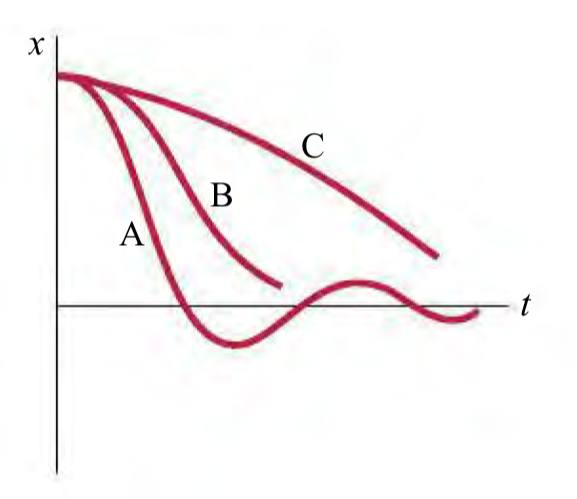
\includegraphics[width=0.4\linewidth]{image/damped-harmonic-motion.png}}
    \end{itemize}
  \item (\textbf{Forced Oscillation: Resonance}) When an oscillating system has an external force applied to it that has its own \textbf{particular frequency}, we have a \textbf{forced oscillation}.
    \begin{itemize}
        \item (\textbf{Its differential equation}) Suppose our $F_{\text{ext}}=F_0\cos\omega t$ and consider the damping force also, we have $\Ddot{x}+\frac{b}{m}\Dot{x}+\omega_0^2x=F_0\cos\omega t$.
        \item (\textbf{Its solution}) Given the initial condition $t=0, x=A$, our general solution is $x=A\cdot e^{-\gamma t}\cdot\cos\omega_0t+A_0\cdot\sin(\omega t+\varphi)$, where $\gamma=\frac{b}{2m}, A_0=\frac{F_0}{m\sqrt{(\omega^2-\omega_0^2)^2+b^2\omega^2/m^2}}, \varphi=\arctan\frac{\omega_0^2-\omega^2}{b\omega/m}$.
        \item (\textbf{Some tips})
        \begin{itemize}
            \item When solving oscillation problems, the first thing is to decide whether it is \textbf{Simple Harmonic Motion}, or \textbf{Damped Harmonic Motion} or \textbf{Forced Oscillation}. Then find the suitable equation to plug in.
            \item When $\omega = \omega_0$, \textbf{resonance} occurs and if damping force is not considered and initial condition is not given, when $\omega = \omega_0$, then our solution becomes $x=A\cos(\omega t+\varphi)+\frac{F}{2\omega}t\sin\omega t$. Otherwise, the oscillator will be \textbf{stable} (means never tend to infinity). Given that the initial condition is \textit{the oscillator starts at rest at equilibrium}, then $A=0$ ($x(0)=0), \dot{x}(0)=0$), a.k.a we can kick out of the first term and now $x=\frac{F}{2\omega}t\sin\omega t$
            \item Notice that in our general solution, as our $t$ increases, the first term approaches 0 because of $Ae^{-\gamma t}$.
            \item The natural frequency of the system $\omega_0$ is called the \textbf{resonance frequency}.
        \end{itemize}
    \end{itemize}
\end{enumerate}

\section{04. The Laplace Transform}
\begin{enumerate}
    \item (\textbf{Definition}) The \textbf{Laplace transform of $f(t)$} is defined by $\mathcal{L}[f(t)]=F(s)=\lim_{h\to \infty}\int_0^he^{-st}\cdot f(t)dt$, and $f(t)$ is the \textbf{inverse} Laplace transform of $F(s)$: $f(t)=\mathcal{L}^{-1}[F(s)]$. (Note that $s$ is a new intermediate variable). \newline
    \centerline{    
    \begin{tabular}{|c|c|}
        \hline
        $f(t)=\mathcal{L}^{-1}[F(s)]$ & $F(s)=\mathcal{L}[f(t)]$
        \\\hline
        $1$ & $\frac{1}{s}$
        \\\hline
        $e^{at}$ & $\frac{1}{s-a}$
        \\\hline
        $\cos at$ & $\frac{s}{s^2+a^2}$
        \\\hline
        $\sin at$ & $\frac{a}{s^2+a^2}$
        \\\hline
        $t^n,n\in N$ & $\frac{n!}{s^{n+1}}$
        \\\hline
        $\delta(t-c)$ & $e^{-cs}$
        \\\hline
        $f(t)\delta(t-c)$ & $e^{-cs}f(c)$
        \\\hline
        $u(t-c)$ & $\frac{1}{s}e^{-cs}$
        \\\hline
        $e^{at}u(t-c)$ & $\frac{e^{-c(s-a)}}{s-a}$
        \\\hline
    \end{tabular}
    }
    \item (\textbf{Linearity}) Given functions $f(t)$ and $g(t)$, $\mathcal{L}[af(t)+bg(t)]=a\mathcal{L}[f(t)]+b\mathcal{L}[g(t)]$ for all $a,b\in R$. Note that $\mathcal{L}^{-1}$ also has \textbf{Linearity}.
    \item (\textbf{Differentiation Property}) $\mathcal{L}[t\cdot f(t)]=-\frac{d}{ds}F(s)$ or $-F'(s)$. General form $\mathcal{L}[t^n\cdot f(t)]=(-1)^nF^{(n)}(s)$, where $F(s)=\mathcal{L}[f(t)]$
    \item (\textbf{First Shifting Theorem}) $\mathcal{L}[e^{at}\cdot f(t)]=F(s-a)$, where $F(s)=\mathcal{L}[f(t)]$
    \item (\textbf{Derivatives}) $\mathcal{L}[y']=s\mathcal{L}[y]-y(0)$, $\mathcal{L}[y'']=s^2\mathcal{L}[y]-sy(0)-y'(0)$. General form is $\mathcal{L}[f^{(n)}(t)]=s^n\mathcal{L}[f(t)]-s^{n-1}f(0)-\cdots-sf^{(n-2)}(0)-f^{(n-1)}(0)$
        \item (\textbf{Second Shifting Theorem}) $\mathcal{L}[f(t-c)\cdot u(t-c)]=e^{-sc}\mathcal{L}[f(t)]$, or $\mathcal{L}[f(t)u(t-c)]=e^{-sc}\mathcal{L}[f(t+c)]$. (Sometimes the later one will be faster!)
    \begin{itemize}
        \item (\textbf{Forward}) Find $u(t-c)$, then use $\mathcal{L}[f(t)u(t-c)]=e^{-sc}\mathcal{L}[f(t+c)]$, then use linearity and other properties to find the corresponding Laplace Transform $\mathcal{L[f(t)]}$, then $t\rightarrow t+c$.
        \item (\textbf{Reverse}) Use $\mathcal{L}^{-1}[e^{-cs}F(s)]=f(t-c)u(t-c)$ Firstly, use the term $e^{-cs}$ to find $c$. Then use the $F(s) \text{ or } \mathcal{L}[f(t)]$ to find $f(t)$. Then, change $t$ to $t-c$.
    \end{itemize}
    \item (\textbf{The method of partial fraction decomposition})
    \begin{itemize}
        \item If the denominator is \textbf{not repeated}, the degree of the \textbf{numerator} should be \textbf{1 less than} the degree of the \textbf{denominator}. e.g. $\frac{1}{s(ms^2+k)}=\frac{A}{s}+\frac{Bs+C}{ms^2+k}$, $\frac{2s^3+4}{s^4+2s^3}=\frac{As^2+Bs+C}{s^3}+\frac{D}{s}$
        \item If the denominator is \textbf{repeated} (a.k.a degree is bigger than 1), start from degree of 1, sum to the current degree. e.g. $\frac{1}{x^2(x^2+1)^2}=\frac{A}{x}+\frac{B}{x^2}+\frac{Cx+D}{x^2+1}+\frac{Ex+F}{(x^2+1)^2}$.
    \end{itemize}
    \item (\textbf{Tips})
    \begin{itemize}
        \item To use the above properties, the first step is to find your $y\text{ or }f(t)$, this is your base function. Then find the Laplace Transform of your base function. Then use the properties.
        \item (\textbf{The Inverse Laplace Transform}) e.g. Evaluate $\mathcal{L}^{-1}[\frac{1+e^{-3s}}{s^4}]$. $F(s)=\frac{1}{s^4}+e^{-3s}\frac{1}{s^4}$. Note that $\mathcal{L}^{-1}[\frac{1}{s^n}]=\frac{t^{n-1}}{(n-1)!}, \mathcal{L}^{-1}[e^{-as}F(s)]=f(t-a)u(t-a)$. Hence, $f(t)=\mathcal{L}^{-1}[F(s)]=\frac{t^3}{3!}+\frac{(t-3)^3}{3!}u(t-3)$
        \item (\textbf{Convolution Integral}) If $\mathcal{L}^{-1}[F(s)]=f(t)$ and $\mathcal{L}^{-1}[G(s)]=g(t)$, then $\mathcal{L}^{-1}[F(s)G(s)]=\int_0^tf(u)g(t-u)du=\int_0^tg(u)f(t-u)du=(f*g)(t)$
        \item (\textbf{Differentiate the unit step function}) For a unit step function $u(t-c)$, if differentiate w.r.t $c$, we treat $u(t-c)$ as a constant.
    \end{itemize}
\end{enumerate}
\subsection{Step Functions and the Unit Impulse}
\begin{enumerate}
    \item (\textbf{Use step function to represent the range})
    \begin{itemize}
        \item $1-u(t-1)$ can represent $t<1$, sometimes it will be $0<t<1$ (depends on the question)
        \item $u(t-1)-u(t-\frac{\pi}{2})$ can represent $1<t<\pi/2$
        \item $u(t-\frac{\pi}{2})$ can represent $t>\pi/2$
    \end{itemize}
    \item (\textbf{Method to get the Laplace Transform of Unit Step Functions}) The idea is to separate the integrals
    e.g. $\mathcal{L}[u(t-c)]=\int_0^\infty e^{-st}u(t-c)dt=\int_0^ce^{-st}u(t-c)dt+\int_c^\infty e^{-st}u(t-c)dt=\int_0^ce^{-st}\cdot0dt+\int_c^\infty e^{-st}\cdot1dt=-\frac{1}{s}e^{-st}|_{t=c}^\infty=\frac{1}{s}e^{-cs}$
    \item (\textbf{Dirac Delta/Unit Impulse Function}) Defined when Impulse $I=1$ and as $\epsilon\to\infty$, the dirac delta function is often used to represent a \textbf{sudden} change in the question and the magnitude/Impulse is 1.
    \item (\textbf{Tips})
    \begin{itemize}
        \item The dirac delta function are defined to be an instantaneous amount of change, but in problems, it should be considered as \textbf{a spike rate of change}!
    \end{itemize}
\end{enumerate}

\section{05. Partial Differential Equations}
\begin{enumerate}
    \item (\textbf{Definition}) A \textbf{partial differential equation} (PDE) is an equation involving one or more \textbf{partial derivatives} of a function that depends on \textbf{two or more variables}.
    \item (\textbf{Linearity and Homogeneity})
    \begin{itemize}
        \item A PDE is \textbf{linear} if it is of the \textbf{first degree} in the \textbf{unknown function and its derivative}. But the \textbf{independent variables} can be of higher degrees. e.g. $u$ is an unknown function of $x,y$, $u\cdot u'=0$ is \textbf{not linear}, $x^2u=0$ is $linear$
        \item A PDE is \textbf{homogeneous} if each of the terms contains either or one of its partial derivatives. (Or, 0 is one of the solutions for the equation)
    \end{itemize}
    \item (\textbf{Solve PDE - Method of separation of variables})
    \begin{enumerate}
        \item Suppose that a solution is given by $u(x,y)=A(x)B(y)$
        \item Rewrite the equation in $A$ and $B$, e.g. $u=AB,u_x=A'B,u_y=AB',u_{xx}=A''B\cdots$
        \item Separate the variables: $f(x, A, A',\cdots)=g(y, B, B', \cdots)$ and let both sides equal to a \textit{separation constant} $k$. Thus, we have two ODEs.
        \item Solve these two ODEs using separation of variables in ODE. Get $A=\cdots x, B=\cdots y$. Then combine these two solutions by $u(x,y)=AB$
    \end{enumerate}
    \item (\textbf{Superposition Principle}) Let $u_1(x,y)$ and $u_2(x,y)$ be solutions of a \textbf{homogeneous linear PDE}. Then, a solution is also given by $u(x,y)=c_1u_1(x,y)+c_2u_2(x,y)$, for any $c_1,c_2\in R$
    \item (\textbf{Solving Tips})
    \begin{itemize}
        \item When using the method of separation of variables, if the PDE becomes an "ODE" (either $A$ or $B$ is eliminated), then after solving the remaining variable, change the constants $c_1,c_2$ to the one that includes the variable that is treated as constants in this PDE, e.g. $f(y), g(y)$
        \item $\int\frac{1}{A}dA=\int(k+1)\frac{1}{x}dx\rightarrow \ln|A|=(k+1)\ln|x|+c$, thus we have $A(x)=c_1x^{k+1}$
    \end{itemize}
\end{enumerate}
\subsection{The Heat Equation}
\begin{enumerate}
    \item (\textbf{Definition}) The dispersion of heat on a metal rod of length $l$ is described by the \textbf{heat equation} $u_t=c^2u_{xx}$, $0<x<l,t>0$. $c^2$ is the \textit{thermal diffusivity of the metal}, and the \textbf{solution} $u(x,t)$ describes the temperature of the rod at a given point $x$ and time $t$. Assuming that at $x=0$ and $x=l$, the rod is insulated, so we have \textit{boundary conditions} $u(0,t)=0,u(l,t)=0$. If the initial distribution of heat is given by the function $f(x)$, then we have the initial condition $u(x,0)=f(x)$
    \item (\textbf{Solution}) The general solution to the heat equation is $u(x,t)=\beta_ne^{-c^2n^2\pi^2t/l^2}sin(\frac{n\pi}{l}x)$, where $c^2,l$ are usually given by question. $n,\beta_n$ are constants that can be derived using the \textit{initial condition},. And by superposition principle, we can divide the initial condition into each $\sin$ function, find its corresponding $n,\beta_n$ and combine them together into one particular solution using superposition principle again.
\end{enumerate}

\end{multicols}
% Dividing Line
\hrulefill \\

\begin{multicols}{3}
\end{multicols}

\end{document}